\newpage
\section{Introduction}

\hbadness=10000
\vbadness=10000

Impacts craters are the dominant landform on the majority of the terrestrial planets. Despite this, there are no eye-witness accounts of crater formation on Earth. 

Forming an impact cratering is a process that not only affects surface morphology, but also strongly influences the evolution of life. For example, it is now widely accepted that a large impact at Chicxulub, Mexico, was the prime reason for the mass extinction event at the Cretaceous-Palaeogene boundary, 66 Ma \citep{schulte2010chicxulub}.

Numerical modelling is a powerful tool for understanding impact crater formation. Model results can be compared to observed crater characteristics, revealing a great deal about the impactor itself, such as its diameter, velocity, angle of impact, and kinetic energy. It is impossible to accurately predict these characteristics from field observations alone. 

During the formation of large impact craters the target rock undergoes a remarkable drop in yield strength relative to static rock measurements. A result of this low yield strength is the formation of a collapsed, terraced crater rim and a central peak/peak ring (Figure \ref{fig:mercurycrater}, \ref{fig:lunarcrater}). Several different models of dynamic weakening attempt to explain this drop in yield strength \citep{kenkmann2012modification}. The aim of this work is to compare and contrast two of these models, the \textit{block oscillation model} \citep{ivanov1997block}, and the \textit{full model of acoustic fluidization} \citep{melosh1979acoustic}.

The block model is itself well tested \citetext{\citet{collins2002hydrocode} and \citet{morgan2000peak}, for example}. For sufficiently large impacts, the block model generates a collapsed rim and central peak/peak ring. However, the weakening generated by the block model is broad and unlocalised. As a result, discrete, terraced fault blocks are never produced, and so current simulations only accurately recreate the broad-scale features of impact crater morphology. 

The full Melosh model of acoustic fluidisation does predict localised weakening through the action of acoustic vibrations \citep{melosh1979acoustic}, and thus may be able to reproduce the localised as well as the broad-scale features of complex craters.

To fully understand the results presented in this work, it is prudent to briefly review the impact process.

\subsection{The Cratering Process}

The process of forming an impact crater is broadly subdivided into three sections; (1) \textit{contact and compression}, (2) \textit{excavation}, and (3) \textit{modification} \citep{osinski2012impact}. 

Contact and compression begins when the impactor makes contact with the surface of the target. Kinetic energy from the impactor is transferred into the target, resulting in both melting/vaporisation and excavation of material near the point of impact \citep{melosh2012contact}. This begins the excavation stage, where material is radially ejected away from the point of impact. Excavation ends when the outward flow of material ceases \citetext{e.g., \citet{osinski2012impact}}. The last stage, modification, is crucial in determining the final crater morphology.

\begin{figure*}[!t]
\begin{minipage}[t]{0.32\linewidth}
\centering
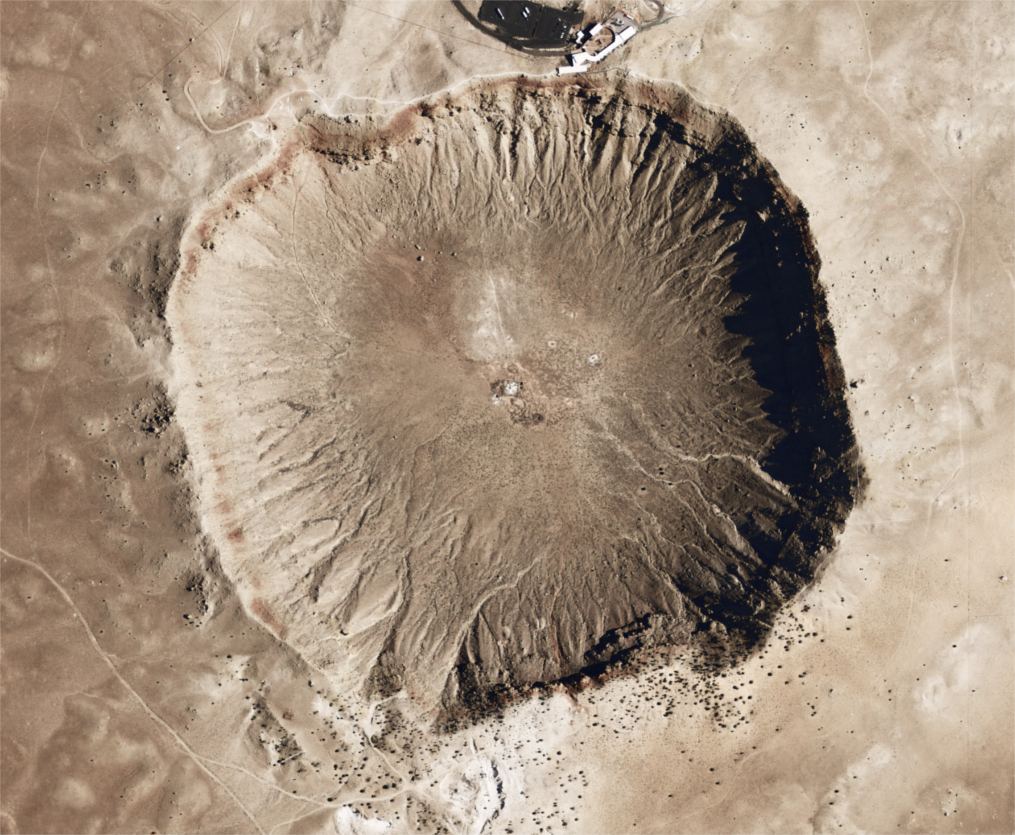
\includegraphics[width=\linewidth]{images/meteor_crater_crop.png}
\subcaption{\textit{Meteor Crater, Arizona}. A classic example of a simple crater on Earth, with a diameter of approximately 1.2km. Image from NASA's aircraft camera instrument. Image credit: NASA Earth Observatory. \url{http://earthobservatory.nasa.gov/IOTD/}. Accessed on December 2nd, 2013. \label{fig:meteorcrater}}
\end{minipage}\hspace*{\fill}
\begin{minipage}[t]{0.32\linewidth}
\centering
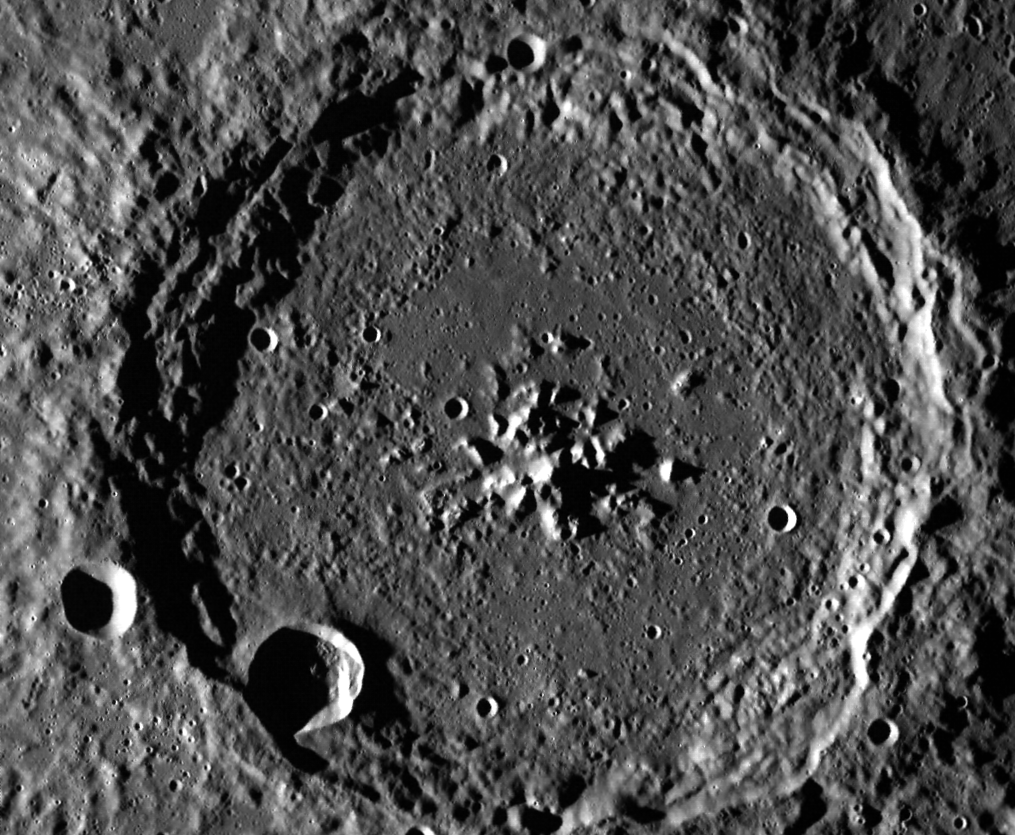
\includegraphics[width=\linewidth]{images/mercurycomplexcrater.png}
\subcaption{\textit{Verdi Crater, Mercury}. A complex crater on the surface of Mercury with a diamater of approximately 144km \citep{hale1980central}. Notice the central peak and collapsed, terraced rim. Image from NASA's Messenger MDIS instrument. Image credit: NASA. \url{http://photojournal.jpl.nasa.gov/}. Accessed on December 2nd, 2013. \label{fig:mercurycrater}}
\end{minipage}\hspace*{\fill}
\begin{minipage}[t]{0.32\linewidth}
\centering
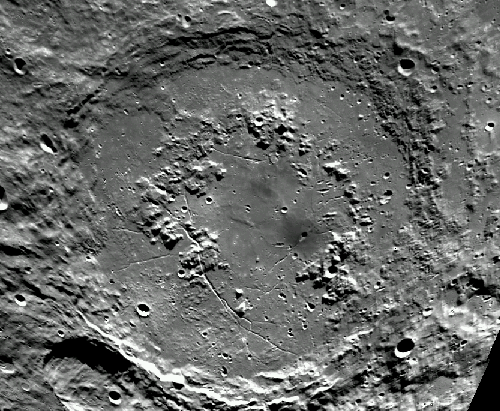
\includegraphics[width=\linewidth]{images/schrodinger.png}
\subcaption{\textit{Schr\"{o}dinger Crater, the Moon}. One of the largest impact craters on the Moon, with a diameter of 320km. At this size, an inner, peak ring is formed rather than a central peak. Image from NASA's Clementine MDIS instrument. Image credit: NASA. \url{http://www.nasa.gov/mission\_pages/Mini-RF/multimedia/}. Accessed on January 3rd, 2014. \label{fig:lunarcrater}}
\end{minipage}
\caption{An example of a simple crater (\protect\subref{fig:meteorcrater}), a  complex central peak crater (\protect\subref{fig:mercurycrater}), and a complex peak ring crater (\protect\subref{fig:lunarcrater}). \label{fig:simplecomplex}}
\end{figure*}

Depending on the size of the impactor, as well as the cohesion and gravity of the target, either a simple (Figure \ref{fig:meteorcrater}) or complex (Figure \ref{fig:mercurycrater} and \ref{fig:lunarcrater}) crater will form. A complex crater is always larger than a simple crater, but has a significantly smaller depth-to-diameter ratio. While a simple crater tends to be bowl shaped, a complex crater often has a flat crater floor with a central peak/peak ring. The rim of a complex crater consists of large terraced blocks of slumped material \citep{osinski2012impact}.

If a crater is large enough at the beginning of modification, it will become gravitationally unstable and collapse \citetext{e.g., \citet{melosh1999impact}}. For collapse to occur, numerical models require that the target rock must be weakened to a much greater extent than standard rock mechanics predicts \citep{mckinnon1978investigation}. Acoustic fluidization \citep{melosh1979acoustic} is a model that attempts to explain this inferred weakening.

\subsection{The Full Model of Acoustic fluidization \label{sec:acfl}}

The full model of acoustic fluidization, derived by \citet{melosh1979acoustic}, is a mechanical model which describes how temporally and spatially varying acoustic vibrations induce temporary weakening.

Acoustic vibrations are generated by the impact's shock wave and are scattered around the impact zone. These vibrations cause pressure fluctuations about the ambient overburden pressure. When the overall pressure drops below the ambient pressure the material's yield strength is reduced, resulting in temporary weakening. Thus, when target deformation is averaged over time and space, the rock material behaves as a viscous fluid. The equation that describes the yield strength of the acoustically fluidized rock material, $Y_{vib}$, is given as \citep{collins2003acoustic}:

\vspace{-0.1cm}
\begin{equation} \label{eq:yield_vib}
Y_{vib} = \eta_{\text{eff}} \dot{\epsilon} \approx  \frac{\rho \lambda c_{p}}{2 \psi} \left[ \frac{1+\erf\left(\chi\right)}{1-\erf\left(\chi\right)} \right] \dot{\epsilon}.\vspace{0.2cm}
\end{equation} 

The basic relationship involves the acoustically fluidized material's strain rate, $\dot{\epsilon}$, and effective viscosity, $\eta_{\text{eff}}$. The full definition of $\eta_{\text{eff}}$ is given on the far right hand side, where $\rho$ is the material's density, $\lambda$ is the wavelength of acoustic vibrations, and $\psi$ is the square of the compressional wave velocity divided by the shear wave velocity, $(c_{p}/c_{s})^{2}$. $\chi$ is defined as \citep{collins2002numerical}: 

\vspace{-0.2cm}
\begin{equation}\label{eq:chi}
\chi=\frac{s_{c}}{\sigma},
\end{equation}

where $s_{c}$ is the critical pressure amplitude for sliding to occur, and $\sigma$ is the variance of the vibrational pressure. $\sigma$ is equal to $c_{p} \rho \sqrt{2E}$, where E is the acoustic energy density (per unit volume). The velocity of the vibrations, $v_{vib}$, is related to the acoustic energy density via \citep{collins2002numerical},

\vspace{-0.2cm}
\begin{equation}\label{eq:velo}
v_{vib}=\sqrt{2E}.
\end{equation} 

The full equation that describes the temporally and spatially varying acoustic energy density per unit time is a non-linear, ordinary differential equation \citep{melosh1996dynamical}:

\begin{equation} \label{eq:dedt}
\frac{d E}{d t} = \frac{\xi}{4} \nabla^{2}E - \frac{c_{p}}{\lambda Q}E + e \tau_{ij} \dot{\epsilon}_{ij},\vspace{0.2cm}
\end{equation} 

where $\xi$ is the scattering diffusivity and $e$ is known as the regeneration parameter. $Q$ is the dissipation quality factor, formally defined as the  ratio of energy stored per cycle to the energy dissipated in that period \citep{collins2003acoustic,melosh1996dynamical}.

The first term on the right hand side of equation \ref{eq:dedt} describes scattering/diffusion of acoustic energy. The effect of the scatter term increases for smaller impacts because the length scale of scattering becomes large with respect to the crater size.
 
The second term describes the conversion of acoustic energy into heat per unit time, hence it is a positive value subtracted from the rate of change of acoustic energy density. It is known as the dissipation term, and is strongly dependent on the product $\lambda Q$. 

The final term in the differential equation acts to generate acoustic energy in regions with large stresses and strain rates. The regeneration parameter, $e$, holds a value between zero and unity, and influences the efficiency of acoustic energy regeneration \citep{melosh1996dynamical}. The term dictates how much distortional energy per unit time (given by $\tau_{ij} \dot{\epsilon}_{ij}$) is converted into acoustic energy.  Without the regeneration term, equation \ref{eq:dedt} would be linear and thus the solution behaviour would be relatively uninteresting. However, the regeneration term causes the equation to become very non-linear, which leads to interesting behaviour.

\subsection{The Block Oscillation Model}

The block model is a widely used alternative to the \citet{melosh1979acoustic} model of acoustic fluidization. It is derived from a simplified situation of acoustic fluidization, where a single block slides over a surface \citep{ivanov1997block}. It assumes that the acoustically fluidized region of the target is fractured into a series of large blocks, each separated by a matrix of smaller blocks. Acoustic vibrations, remnant from the impact's shock wave, cause the larger blocks to oscillate, decreasing the stress and coefficient of friction between the blocks and the matrix \citep{collins2002numerical,ivanov1997block}. Consequently, sliding is induced between the blocks.

The effective strength of the rock material for the block model, $Y_{\text{eff}}$, is given as:

\begin{equation}
Y_{\text{eff}}=\mu (p-p_{v}) + \eta_{\text{eff}} \dot{\epsilon}
\end{equation}

where $\mu$ is the coefficient of friction, $p$ is the overburden pressure and $p_{v}$ is the amplitude of the pressure vibrations from the sliding blocks \citep{ivanov1997block,melosh1999impact}. In contrast to the Melosh model, $\eta_{\text{eff}}$ is an input parameter rather than a function of acoustic energy. For the block model, it is assumed that $\eta_{\text{eff}}$ is proportional to impactor size. \citet{melosh1999impact} showed that the rheological effects of the block and Melosh models are similar. 

The block model, as implemented in the impact model used here, effectively solves equation \ref{eq:dedt} from the Melosh model for the case $e=0$ and $\xi=0$, so scattering and (re)generation of acoustic energy are never applied. Thus, the block model only solves the dissipation of acoustic energy. The initial distribution of acoustic vibrations, as implemented here, is based on the peak particle velocity of the target rather than through the regeneration term, thus initial acoustic vibrations follow the path of the shock wave. 

The block model fails to induce distinct, fault sized zones of localised weakening into hydrocode simulations \citep{kenkmann2012modification} because it neglects the scattering and, in particular, regeneration terms from equation \ref{eq:dedt}.

\subsection{The iSALE Hydrocode}

The impact model used to simulate crater formation in this research is known as iSALE, developed by Kai Wuennemann, Gareth Collins, and Dirk Elbeshausen. iSALE is a model for simulating flow at all speeds, including hypersonic flows and shock waves, otherwise known as a hydrocode \citep{collins2002numerical}. Essentially, a hydrocode calculates the sum of all forces acting at a node, and applies the corresponding acceleration to either the node or material within a cell, depending on an Eulerian or Lagrangian frame of reference, respectively. This process is carried out iteratively over all nodes in the model domain at incremental time steps. When the sum of all time steps reaches the final simulation time, the calculations stop \citep{collins2002numerical}.

iSALE is well suited for simulating asteroid impacts because it includes strength models that take into account the rheological properties of the medium. This is very important for impact cratering; the final, modified crater hugely depends on the rheology of the target, which may change depending on the size, velocity, and strength of the impactor, among other factors.
